\documentclass[a4paper,11pt,hidelinks]{article}
%\usepackage[a-1b]{pdfx}
\usepackage{hyperref}
\usepackage{bookmark}

\usepackage{subfiles}
\usepackage{epsfig}
\usepackage{plain}
\usepackage{setspace}
%\usepackage{minted}
\usepackage{mdframed}
\usepackage{caption}
\usepackage{color}
\usepackage{amsmath}
\usepackage{amsthm}
\usepackage{amssymb}
\usepackage{amsfonts}
\usepackage{mathabx}
\usepackage{tcolorbox}
\usepackage{multicol}
\usepackage[english]{babel}
\usepackage[left=2cm,right=2cm,top=2cm,bottom=1.8cm]{geometry}
\usepackage{titlesec} 
\usepackage[utf8x]{inputenc} 

\newtheorem{theorem}{Theorem}
\newtheorem{corollary}{Corollary}[theorem]
\newtheorem{lemma}{Lemma}[theorem]

\hypersetup{colorlinks=false, urlcolor=blue}

\captionsetup{
  justification=centering,
  singlelinecheck=false,
  font=small,labelfont=bf,labelsep=space}

\begin{document}

\pagestyle{plain}

\begingroup

\renewcommand{\cleardoublepage}{}
\renewcommand{\clearpage}{}

\titleformat{\section}
{\normalfont\Large\bfseries}{\thesection}{1em}{}

\newpage

\title{Impossibility of Distributed Consensus}
\author{Distributed Systems 2 \\
    (original author: Alberto Montresor \texttt{<alberto.montresor@unitn.it>}) \\
    Matteo Franzil \texttt{<matteo.franzil+github@gmail.com>}}
\maketitle

\tableofcontents

\newpage

\section{Impossibility Result}

\subsection{Problem Description}

The problem of consensus can be formulated as following:

\begin{itemize}
    \item n processes, each of them proposes a value;
    \item they must decide, reaching an agreement, one of the proposed values.
\end{itemize}

In this paper, we analyze the result given by the paper by Fischer, Lynch, Paterson \cite{10.5555/889891}, that says that no algorithms can solve consensus in an asynchronous distributed system in which a single process may crash. Another important paper in the literature is the one by Chandra and Toeug \cite{10.1145/234533.234549}, that shows how consensus can be solved in asynchronous distributed systems provided with a failure detector, even if processes may crash.

The first paper has a strong system model, but faulty processes and weak consensus model; the opposite is true for the second paper.

The point of all of this is that it's easy to reach a decision (well, at least theoretically) when the networks and the processes are perfectly functioning, but in real distributed systems, both can fail and lead to weird results. In particular, for the moment we will analyze the case of normal crash and omission failures, and not Byzantine failures. Still, we are not able to solve the problem even with normal failures!

\subsection{Preliminaries}

\begin{itemize}
    \item $\Pi = {P_1, \cdots, P_n}$ is the set of processes
    \item Each process $p_i$ executes \verb=propose(=$v_i$\verb=)= proposing a value $v_i$
    \item Each process p can execute an action \verb=decide(=$v$\verb=)= in which value $v$ is decided.
    \item The set of possible values is just {0, 1}.
\end{itemize}

\noindent Properties:

\begin{itemize}
    \item \textbf{Termination}: Eventually, each correct process decides for some value.
    \item \textbf{(Uniform) Agreement}: All correct processes (all processes) that decide, decide for the same value.
    \item \textbf{Uniform Validity}: If a process decides $v$, then $v$ has been proposed by some process.
    \item \textbf{Uniform Integrity}: Each process decides at most once.
\end{itemize}

\noindent System model:

\begin{itemize}
    \item Asynchronous distributed system:
          \begin{itemize}
              \item No upper bound to message delays
              \item No upper bound to relative process speeds
              \item No synchronous clocks
          \end{itemize}
    \item All processes know the $\Pi$ set.
    \item No communication failures
    \item At most one crash failure, with the crashed process stopping executing actions
\end{itemize}

We can assess that no matter what protocol, bad or good, we come up with, we can get a contradictory results. Examples of bad protocols include ones in which processes decide all 0 or 1, majority ones, and more.

\noindent Notation:

\begin{itemize}
    \item $P_i$ is an infinite deterministic automata
    \item $\sigma_i$ is the internal state of the process $P_i$
          \begin{itemize}
              \item $IN_i \in \{0, 1\}$ is the initial proposed value
              \item $OUT_i \in \{0, 1\}$ is the decided value and is write-once
          \end{itemize}
    \item a state is called initial if $OUT_i = \bot$, else it is a decision state
\end{itemize}

\noindent Regarding the communication, we have:

\begin{itemize}
    \item $B$: a magic Internet buffer, akin to a perfect channel
    \item \verb=send(=$m, q$\verb=)= $\Rightarrow$ $B = B \cup \{\langle q, m \rangle\}$
    \item $r = $ \verb=receive(=\verb=)= that \textit{nondeterministically} either outputs:
          \begin{itemize}
              \item $r = m$ if $(p, m) \in B$, therefore $B = B - \{\langle p, m \rangle\}$
              \item $\bot$ if there's nothing for the process
          \end{itemize}
\end{itemize}

\noindent We must remember that we're dealing with perfect channels, so \verb=receive()= will eventually deliver each pair to the intended destination. Finally, some more definitions on our event system:

\begin{itemize}
    \item $C = \sigma_1 \cdots \sigma_m \cup B$ is a configuration, i.e., a global state consisting of all states of each processes and the magic buffer $B$. If each state is the initial state (and the buffer is empty), the configuration is called initial.
    \item $e = (p_i, m)$ is an event, that brings the system to a configuration $C \Rightarrow^e C'$ with a primitive step of the process itself.
    \item $s = e_i \cdots e_k$ is a schedule, i.e., a series of events that are orderly applied to a process: \\ $e_k(e_{k-1}(\cdots e_2(e_1(p_i))))$
    \item Each configuration has a decision value $v$ if $\exists p_i \in \Pi : OUT_i = v \and v \ne \bot$.
    \item A run is a potentially infinite schedule that
          \begin{itemize}
              \item is called \textbf{admissible} is there is at most a faulty process and all messages are eventually delivered
              \item is called \textbf{deciding} if at the end a value is decided
          \end{itemize}
\end{itemize}

\noindent Our system is very powerful and extensible: we consider only 0/1 decisions (but can be easily adapted) and the set of processes is globally known. Still, our system is asynchronous, and this will cause some issues.

\subsection{Theorem}

\begin{theorem}[Impossibility of Distributed Consensus]
    No consensus protocol is totally correct if a single crash is possible.
\end{theorem}

We prove the theorem by contradiction: we assume that a totally correct protocol P exists, and we derive a contradiction.

Let $C$ be a configuration and let $V(C)$ be the set of decision values in the decision configurations reachable from C:
\begin{itemize}
    \item If $V(C) = \{0\}$, C is 0-valent
    \item If $V(C) = \{1\}$, C is 1-valent
    \item If $V(C) = \{0, 1\}$, C is bivalent
    \item If $V(C) = \varnothing$, not possible (P is totally correct).
\end{itemize}

\noindent We will prove this theorem with the following plan:

\begin{enumerate}
    \item We prove that P has a initial bivalent configuration
    \item We prove that is always possible to go from a bivalent configuration to a bivalent configuration
\end{enumerate}

We want to prove that given any protocol we can create an infinite loop of going from bivalent to bivalent configuration and thus a decision is never made.

\begin{figure}[!h]
    \centering
    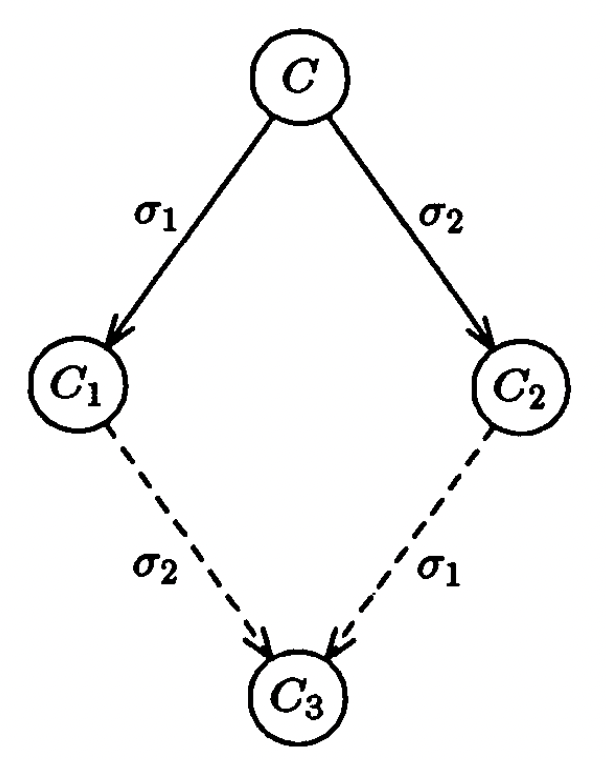
\includegraphics[width=0.33\textwidth]{drawable/fig1.png}
    \caption{Lemma 1}
    \label{fig1}
\end{figure}

\begin{lemma}[Schedule Commutativity]
    Assume that from configuration $C$ the schedules $s_1$ and $s_2$ bring to configurations $C_1$ and $C_2$, respectively. If the sets of processes that execute actions in $s_1$ and $s_2$ are disjoint, then $s_1$ can be applied to $C_2$ and $s_2$ can be applied to $C_1$ and both lead to the same configuration $D$:

    $$
        \{ p_i | (p_i, m) \in s_1\} \cap \{p_j | (p_j, m) \in s_2\} = \varnothing \Rightarrow s_2(C_1) = D = s_1(C_2)
    $$

\end{lemma}

The proof follows from the definition of applicability, as $s_1$ and $s_2$ do not interact.

\begin{theorem}[Bivalent Initial Configuration]
    P has a bivalent initial configuration. Informally, it means that for some initial states, the final decision is not deterministically decided by the value of the proposed values, but it depends on the order in which messages are received.
\end{theorem}

\begin{proof}
    By contradiction, let us assume that P does not have initial bivalent configurations.

    \begin{itemize}
        \item All initial configurations are either 0-valent or 1-valent. Each initial configuration could be described by a binary string of proposed values, such as $1000 \cdots 0$. $P$ must have both 0-valent and 1-valent initial configurations ($00 \cdots 00$ and $11 \cdots 11$); if not, validity would be violated. A pair of initial configurations are said adjacent if their strings differ by a single bit. Example: 1000 and 1100. Each pair of initial configurations is linked by a chain of initial configurations, each adjacent to the next. E.g. 0000 - 1000 - 1100 - 1110 - 1111.
        \item Let us consider a chain of initial configuration, where the first is 0-valent and the last is 1-valent. In this chain, there should be two initial configurations adjacent to each other, one 0-valent ($C_0$) and the other 1-valent ($C_1$).
        \item Let $p_i$ be the process whose proposed value differs in the two configurations. Let $R$ be an admissible, deciding run from $C_0$ in which $p_i$ never executes steps (it is faulty), and let $s$ be the associated schedule. We know that $s$ can be applied also to $C_1$. Indeed, $s(C_0)$, $s(C_1)$ differ only for the initial value of p0, which is faulty, so the decision in $s(C_1)$ is equal to $s(C_0)$; if this decision is 1, in reality $C_0$ is bivalent, else if this decision is 0, in reality $C_1$ is bivalent. In both cases, we obtained a contradiction.
    \end{itemize}
\end{proof}

\begin{theorem}[Bivalent Configuration to Bivalent Configuration]
    P can move from any bivalent configuration to any bivalent configuration.
    \begin{itemize}
        \item Let $C$ be a bivalent configuration
        \item Let $e = (p_i, m)$ be an event applicable to $C$
        \item Let $\hat{C} = \{s(C) | e \notin s\}$ be the set of configurations reachable from $C$ without applying $e$;
        \item Let $\hat{D} = e(\hat{C}) = \{e(C_0) | C_0 \in \hat{C}\}$ be the set of configurations reachable from the configurations of $\hat{C}$ by applying $e$. Then $\hat{D}$ contains a bivalent configuration.
    \end{itemize}
\end{theorem}

\begin{proof}
    By contradiction; $\hat{D}$ does not contain bivalent configurations.

    \medskip

    \noindent\textbf{Part 1.}

    \medskip

    First, we prove that $\hat{D}$ contains both 0-valent and 1-valent configurations. We know that:

    \begin{itemize}
        \item $\hat{D}$ does not contain any bivalent configurations (by contradiction)
        \item $e$ is applicable to $C$ implies that e is applicable to each $E \in \hat{C}$
        \item Let $E_i$ be a i-valent configuration reachable from $C$ $(i = 0, 1)$; $E_i$ exists because C is bivalent;
    \end{itemize}

    The situation can be depicted in this way:

    $$
        \text{0-valent      } E_0 \xleftarrow{s_0} C \xrightarrow{s_1} E_1 \text{      1-valent}
    $$

    There are two possibilities:

    \begin{itemize}
        \item 1st case: $E_i \in \hat{C}$; the situation can be depicted like this:
              $$
                  C \xrightarrow{s_i} E_i \xrightarrow{e} F_i
              $$
              where $E_i$, $F_i$ are i-valent, $E_i \in \hat{C}, Fi \in \hat{D}$.
        \item 2nd case: $E_i \notin \hat{C}$; the situation can be depicted like this:
              $$
                  C \rightarrow \bullet \xrightarrow{e} F_i \rightarrow E_i
              $$
              where the whole succession is a schedule $s$, $E_i$ is i-valent; $F_i$ is not bivalent, is not $(1−i)$-valent, so it is i-valent. Therefore, $F_i \in \hat{D}$.
    \end{itemize}

    \medskip

    \noindent\textbf{Part 2.}

    \medskip

    We want to prove that: There are two configurations $C_0, C_1 \in \hat{C} : C_1 = e'(C_0) : e(C_i) = D_i$ is i-valent and $D_i \in \hat{D}$.

    There are two cases: $e(C) \in \hat{D}$ can be 0-valent or 1-valent. Let assume that $e(C)$ is 0-valent (the other case is symmetrical).

    Let s be a schedule such that:
    \begin{itemize}
        \item $s(C) \in \hat{C}$ (means: $e \notin s$)
        \item $e(s(C))$ is 1-valent (based on Part 1, there is one)
        \item $s = e_1 e_2 \cdots e_n$.
    \end{itemize}

    We get:

    \[
        \begin{array}{ll}
            e(C)                               & \text{0-valent}, \in \hat{D} \\
            e(e_1(C))                          & \text{0-valent}, \in \hat{D} \\
            D_0 = e(e_2(e_1(C))) = e(C_0)      & \text{0-valent}, \in \hat{D} \\
            D_1 = e(e_3(e_2(e_1(C)))) = e(C_1) & \text{1-valent}, \in \hat{D} \\
            \cdots                             & \text{1-valent}, \in \hat{D} \\
            e(s(C))                            & \text{1-valent}, \in \hat{D} \\
        \end{array}
    \]

    In other words, we have found $C_0$ and $C_1$ of the claim.

    \begin{figure}[!ht]
        \centering
        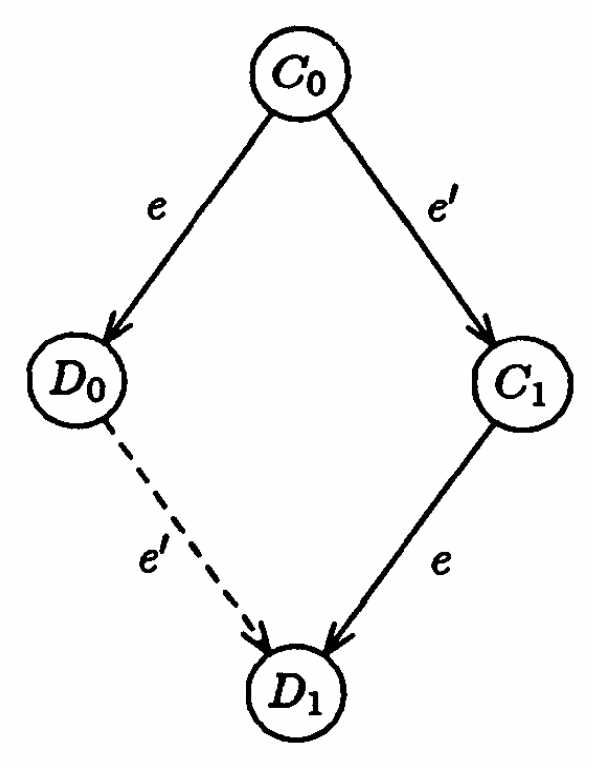
\includegraphics[width=0.33\textwidth]{drawable/fig2.png}
        \caption{Lemma 2, part 3, case $p_i \ne p_j$}
        \label{fig2}
    \end{figure}

    \begin{figure}[!ht]
        \centering
        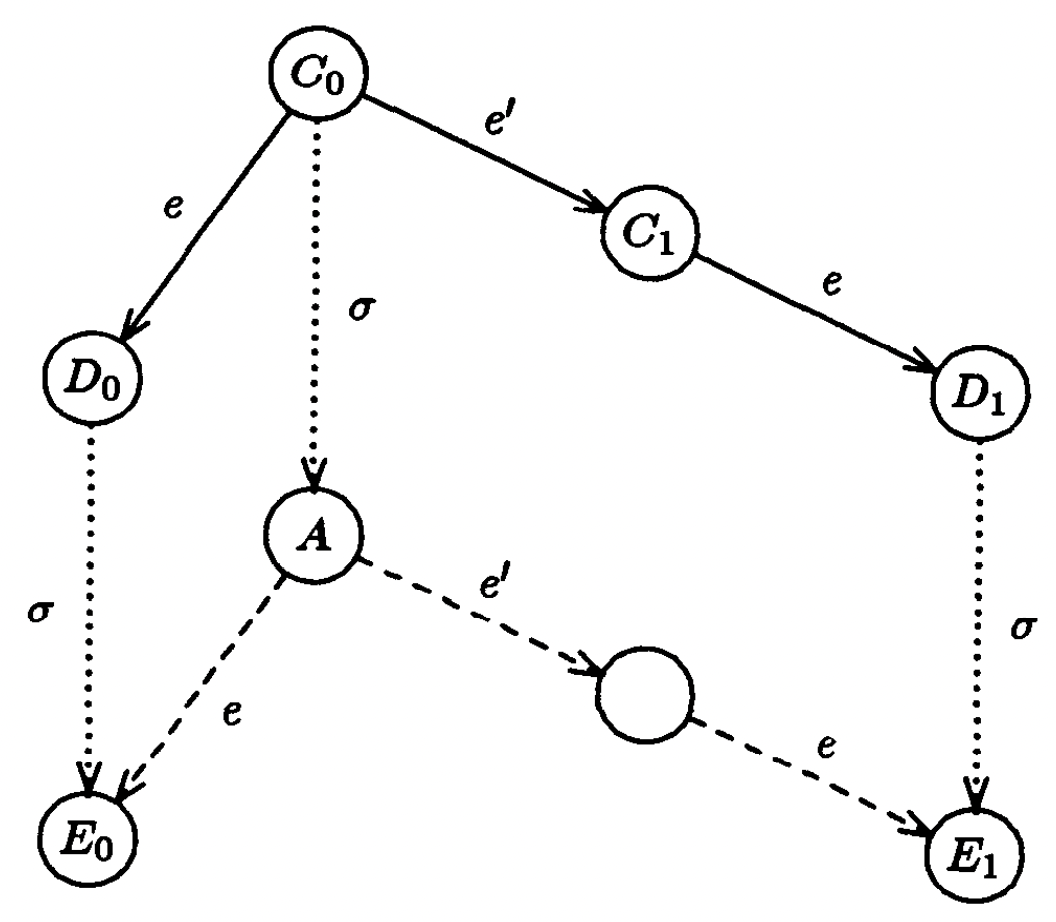
\includegraphics[width=0.33\textwidth]{drawable/fig3.png}
        \caption{Lemma 2, part 3, case $p_i = p_j$}
        \label{fig3}
    \end{figure}

    \medskip

    \noindent\textbf{Part 3.}

    \medskip

    Let $C_0, C_1 = e'(C_0) : e' = (p_j, m')$; we know that $C_0, C_1 \in \hat{C}; D_i = e(C_i)$ is i-valent. There are two possibilities:

    \begin{itemize}
        \item $p_i \notin p_j$: it is possible to apply Lemma 1, and we obtain the diamond of Figure \ref{fig2}. This is a contradiction, because any successor of a 0-valent configuration is 0-valent.
        \item $pi = pj$: Let $\sigma$ be a deciding schedule in which $p_i$ never executes any event (for example, because it becomes faulty); such schedule exists because of total correctness.
              From Lemma 1, $\sigma$ is applicable to $D_0$ and $D_1$. But this is a contradiction, because from A we can reach both $D_0$ and $D_1$, which are 0-valent and 1-valent; so A is bivalent, but this is impossible, because $\sigma$ is a deciding run.
    \end{itemize}

    What does it mean? That given a bivalent configuration, any decision based
    on the observation that a given process $p_i$ is crashed, can be contradicted by a later action of process $p_i$.
\end{proof}

\subsection{Conclusion}

We prove now that given a totally correct protocol P, it is always possible to build an admissible run which is not deciding; a contradiction. We cannot “crash” more than one process; which means that the other processes must execute an infinite number of actions.

Elements:

\begin{itemize}
    \item A process queue $p_1 p_2 p_3 \cdots p_n$
    \item A message queue ordered by sending time. The building is based on stages; ad each stage, we make one of the process execute an action (none of them crash).
    \item Stage 0: We select an initial bivalent configuration $C_0$ (Lemma 2)
    \item Stage i: We select an event $e_i = (p, m)$ where \begin{itemize}
              \item $p_i$ is the first process in the queue
              \item $m$ is the first message for $p_i$
              \item $\bot$ if none present
          \end{itemize}
    \item Using Lemma 3, we build a bivalent configuration $C_i$ starting from $C_{i−1}$ and $e_i$.
    \item We remove the process from the front of the queue and we re-insert it at the end.
\end{itemize}

Final results:

$$
    C_0 \xrightarrow{s_1} \bullet \xrightarrow{e_1} C_1 \xrightarrow{s_2} \bullet \xrightarrow{e_2} C_2 \rightarrow \cdots
$$

Infinite run, with no process failures, in which we never decide.

\section{Beyond Impossibility Results}

Assume we now want to adapt the model in order to make its implementation feasible. Indeed, the model and the properties are the same as the ones described as before. Consensus in such systems is impossible, even if at most a process crashes and the links are reliable. So, either we change the specification or we change the model (better!). This allows us to conceive what is the minimal set of requirements for correctly building a consensus model.

We design our protocol in order to be first safe, then with liveness. In order to move towards our goal, we can add randomized algorithms, failure detectors, or both. They are called \textit{oracles}, and they are modular, in the sense that their design is independent of the algorithm we're adapting it to.

\subsection{Failure detectors}

A failure detector is a distributed oracle whose goal is to tell processes \textit{hints} about the state of other processes in the systems (if they're up or down). But hints may be incorrect, the FD may give different data to different processes, or change its mind several times.

Then why we use unreliable detectors? We abstract everything and use a modular decomposition, so that its properties can be used to show correctness no matter what the situation. In other words, if the algorithm works in this unreliable situation, it always works.

What is the weakest failure detector needed to solve the problem (in an asynchronous system)?

Let us assume the existence of a global clock, not accessible by the single processes. A failure pattern is a function $F: \mathcal{T} \rightarrow 2^{\Pi}$, where $F(t)$ is the set of processes that have crashed through time t: $\forall t \in T: F(t) \subseteq F(t+1)$

The crashed set is the union of $F(t)$ over all the ticks, and the correct set is its complement.

A failure detector history is a function $H: \Pi \times \mathcal{T} \rightarrow 2^{\Pi}$, where $H(p, t)$ is the output of the failure detector of process $p$ at time $t$. If $q \in H(p, t)$, then we say $p$ suspects $q$ at time $t$ in $H$.

The idea of suspicion is backed up by two properties, completeness and accuracy. Completeness may be either strong (if every faulty process is permanently suspected by every correct process) or weak (if only some processes will do eventually).

\begin{align}
    \textit{(strong)}\quad\quad \forall F, & \forall H, \exists t \in \mathcal{T} , \forall p \in crashed(F), \forall q \in correct(F), \forall t' \ge t : p \in H(q, t') \\
    \textit{(weak)}\quad\quad \forall F,   & \forall H, \exists t \in \mathcal{T} , \forall p \in crashed(F), \exists q \in correct(F), \forall t' \ge t : p \in H(q, t')
\end{align}

On the other hand, accuracy tells us that \textit{every} correct process is never suspected. The weak version tells us that \textit{some} correct process is never suspected.

\begin{align}
    \textit{(strong)}\quad\quad \forall F, & \forall H, \forall \in \mathcal{T}, \forall p \in correct(F), \forall q: p \notin H(q, t) \\
    \textit{(weak)}\quad\quad \forall F,   & \forall H, \forall \in \mathcal{T}, \exists p \in correct(F), \forall q: p \notin H(q, t)
\end{align}

The eventual versions of strong accuracy and weak accuracy tells us that unlike never, processes get suspected \textit{eventually}.

By mixing and matching accuracy and completeness, we can get different flavours of failure detectors. As a general idea, strong completeness and accuracy yields \textit{perfect} FDs, weak accuracy and strong completeness yield \textit{strong} FDs (the opposite is not important for us), weak and weak yield \textit{weak} FDs. We can build reductions between them, and in particular reduction from $P$ to $S$ to $W$, and from them to their eventual versions (called $\diamond P/S/W)$). Using another reduction, we can for example jump from weak to strong completeness - the opposite of before, and also for the eventual version, and we can show they're actually equivalent: $W \ge S, S \ge W \Rightarrow S \equiv W$.

\subsubsection{Back to reliable broadcast}

We can modify our reliable broadcast to add eventual strong failure detectors ($\diamond S$). If a process is faulty, then it is inserted into a set of sussy processes by the detector, and the processes eventually receive this information (correctly) by the detector, and will alert the original process. Else, if the process is correct, the message will arrive as it is since the channels are perfect.

In order to properly implement this in our reliable broadcast, we need an eventually perfect FD as accurate as possible in order to reduce the number of re-transmissions (since it's usually linear without crashes, but explodes if someone does not report).

However, is perfect failure detection really necessary? The answer is no! Even eventually strong failure detectors at first output arbitrary information, but given the eventuality, there a time in which every process that crashes is suspected, and some process that does not crash is suspected. If $f < \frac{n}{2}$, $\diamond S$ is necessary and sufficient to solve consensus. Also, remember that $\diamond S \equiv \diamond W$

\subsubsection{Rotating coordinators}

The protocol described here is based on Most{\'e}faoui and Raynal \cite{10.1007/3-540-48169-9_4}

Assume we have processes are numbered $0, 1, \cdots, n - 1$. They execute asynchronous rounds. In round $r$, the coordinator - which corresponds to process $r mod n$ - tries to impose its estimate as the consensus value. It succeeds if does not crash and it is not suspected by $\diamond S$.

With $\diamond S$, no process blocks forever waiting for a message from a dead coordinator. Given that $f < n/2$, eventually every node will receive more than $\lfloor n / 2 \rfloor$ messages and will exit from Phase 2. But since our model is eventual, some correct process $p_c$ will be not falsely suspected (eventually). When it will be his turn, every correct process will receive $c$'s estimate and will decide. This assures us that the process will terminate.

Assume a process $p$ decides $v$ and then crashes. It did so because a majority of messages and decided $v$. Then eventually, another process will decide $v$, since the two majorities important for the decision have their intersection not empty (due to definition of majority).

But what if the FD misbehaves? Well, we cannot satisfy accuracy: the word \textit{eventually} has a very strong connotation, which is in stark contrast with \textit{never}. If a process stays correct in a period of time long enough for the completion of the protocol, then it will succeed. Still, the algorithm remains safe (as completeness is always satisfied), we just have to wait for a good FD period.

An \textbf{indulgent algorithm} - such as the one above - is one that never violates the safety property and rather terminates in case of problems with FDs.

Slides give an insight on possible practical applications of the protocol.

\subsection{Randomization}

Randomization is another approach for solving consensus, which changes the underlying model. Assume we need to solve binary consensus. This protocol achieves probabilistic termination, with $f$-correctness ($f < n/2$), and upper bound $O(2^{2n})$.

\subsubsection{Ben-Or's Algorithm}

This algorithm operates in rounds, each round has two phases:
\begin{itemize}
    \item Report phase - each process transmits its value, and waits to hear from other processes
    \item Decision phase - if majority found, take its value; otherwise, flip a coin to change the local value
\end{itemize}

The idea is based on the fact that if enough processes detected the majority, decide. If I know that someone detected majority, switch to the majority’s value; otherwise, flip a coin. Eventually, a majority of correct processes will flip in the same way.
\medskip\\
\noindent \textbf{Uniform Agreement}: At most one value can receive majority in the first phase of a round.
\begin{itemize}
    \item if some process sees $f + 1$ $\langle proposal, r, v \notin i \rangle$, then every process sees at least one $\langle proposal, r, v \notin i\rangle$ message
    \item if every process sees at least one $\langle proposal, r, v \notin i\rangle$ message, then \begin{itemize}
              \item every process changes its estimate to v
              \item every process reports $v$ in the first phase of round $r + 1$
          \end{itemize}
    \item if every process reports $v$ in the first phase of round $r + 1$, every process decides $v$ in the second phase of round $r + 1$
\end{itemize}
\textbf{Validity} If there are two distinct values at the beginning, one of them will be chosen
\begin{itemize}
    \item Otherwise, if all processes report their common value $v$ at round 0, then: \begin{itemize}
              \item all processes send $\langle proposal, 0, v\rangle $
              \item all processes decide on the second phase of round 0
          \end{itemize}

\end{itemize}
\textbf{Termination}: If no process sees the majority value, then they all will flip coins, and start everything again.
\begin{itemize}
    \item Eventually a majority among the correct processes flips the same random value: \begin{itemize}
              \item The correct processes will observe the majority value.
              \item The correct processes will propagate proposal messages, containing the majority value
          \end{itemize}

    \item Correct processes will receive the proposal messages, and the protocol finishes
\end{itemize}

Finally, these two approaches can be combined in a hybrid system. During bad FD periods, the coin flip system can be made available to processes in order to let processes continue and try to make a decision quicker.

\endgroup

\newpage

\addcontentsline{toc}{section}{Bibliography}

\bibliographystyle{apalike}
\bibliography{biblio}

\end{document}